% ======================================================================
% 第四章：研究結果（研究一：文獻證據；研究二：專利證據）
% 譯自 paper/en/studies.tex（英文稿第 4、5 節）。所有數字與英文稿及 raw_materials/experimental_log.md 一致。
% ======================================================================

\chapter{研究結果}
\label{zh:ch:results}

\section{研究一：文獻證據}
\label{zh:sec:study1}

研究一是結構洞（structural hole）前提最初被提出的研究脈絡。其專案版本標記為 V5--V11.1，僅用於將結果對應至專案紀錄：V5 建立文獻語料庫，V9 為 AI 家族 $\times$ 決策家族矩陣的凍結分析，V6--V11.1 則為網路分析脈絡。本研究連同 2026 年 11 月 18 日的資料效度再分析一併報告研究一；該再分析並未預先登錄（preregistration）。除標示為 HISTORICAL／USER\_REPORTED 者外（第~\ref{zh:sec:study1_network}~節），各數字的來源等級（provenance grade）皆為 DIRECT。

\subsection{語料庫、編碼與檢定設計}
\label{zh:sec:study1_corpus}

語料庫包含 2,118 份來源文件，其中 1,729 份完成剖析。剖析共產生 26,501 筆候選證據紀錄，其中 6,499 筆符合嚴格納入篩選條件。LLM 處理流程將每一個證據句歸入 10 個 AI 家族之一與 12 個決策家族之一，結果為一個含 120 格的二分網路（bipartite network）矩陣。在每份文件內去除重複後，得到 2,180 條文件層級的邊。120 格中有 104 格有觀察值；16 個零值格與下文所報告的 16 個偏低格（depleted cells）互不重疊。多數的邊（86.5\%）來自 AI 軌文件。對於邊際度數分別為 $k_a$ 與 $k_d$ 的 AI 家族 $a$ 與決策家族 $d$，期望次數為
\begin{equation}
E_{ad} = \frac{k_a\,k_d}{M}, \qquad M = 2{,}180 .
\label{zh:eq:s1_expected}
\end{equation}

每一格皆以四項檢定評估：
\begin{enumerate}
  \item 固定度數的端點重配蒙地卡羅（stub Monte Carlo）虛無模型（null model）（$R = 10{,}000$；種子 20260918）；
  \item 精確超幾何檢定（exact hypergeometric test）；
  \item 保留文件結構的文件內交換 MCMC（document-preserving swap null），於 V9 引擎中標記為 M06（5,000 個樣本，預燒期 43,600，抽稀間隔 4,360；種子 20260919）；
  \item 以未去除重複之紀錄進行的原始紀錄精確檢定（raw-record test）（$n = 3{,}125$）。
\end{enumerate}
Benjamini--Hochberg（BH）程序在 120 格內控制偽發現率（false discovery rate, FDR）\citep{benjamini1995controlling}。一格須同時符合下列條件，方納入凍結的\emph{核心格}（core）：在主要檢定、精確檢定與保留文件結構檢定中皆為 $q \le .05$ 且三者方向一致，另原始紀錄檢定亦須 $q \le .05$ 且方向相同。共有 32 格符合此規則，其中 16 格偏高、16 格偏低。「偏低」與「偏高」（enriched）是相對於上述虛無模型的統計描述，並非分隔（separation）的證據，本研究亦不將偏低格稱為缺口（第~\ref{zh:sec:design_boundaries}~節）。

以下兩項性質限定了其後的所有結果，包括專利類比分析（第~\ref{zh:sec:study2_cells}~節）：其一，精確檢定與原始紀錄檢定忽略文件內群聚（clustering）；其二，核心格結合了各檢定內的 BH 校正與相依檢定之間的一致性，因此並無單一明確定義的偽發現率，應解讀為一種保守的篩選（第~\ref{zh:sec:lim_inference}~節）。

\subsection{偏低格的方向與穩健性}
\label{zh:sec:study1_direction}

表~\ref{zh:tab:app_v9cells} 列出 16 個偏低格及其觀察次數。最極端者為 \texttt{PREDICTION\_\allowbreak RISK\_\allowbreak ESTIMATION}~$\times$ \texttt{HUMAN\_\allowbreak REVIEW\_\allowbreak ACCOUNTABILITY}，其 $O = 6$，而 $E = 44.9$。

\paragraph{計算穩健性。} 以獨立重新實作的精確檢定與原始紀錄檢定，可在 $|\Delta q| \le 6\times10^{-12}$ 的誤差內重現官方的 $q$ 值。32 格核心格的 Jaccard 重疊為 .94。在 20 個蒙地卡羅種子下，有 31 格在每一個種子下皆屬核心格，其中包括全部 16 個偏低格。其餘 2 個邊界格，恰為先前一次經人工校正之重新編碼所識別出的「一進一出」配對。

\paragraph{組成穩健性。} 在固定 AI 軌與決策軌文件組成的分軌分層虛無模型下，16/16 個偏低格與 16/16 個偏高格仍維持顯著且方向不變，故此型態並非 AI 軌文件居多所造成的假象。來自偏低核心格的紀錄通過嚴格篩選的比例高於來自其他格的紀錄（38\% 對 28\%）。

\paragraph{時間穩健性。} 圖~\ref{zh:fig:study1_direction} 將文件分為 2023 年（含）以前與 2024 年（含）以後兩期。全部 16 格在兩期中皆為偏低（16/16），且兩期之間的變化與置換虛無模型並無差異（$p = .86$）。因此，此一不足在兩期中方向相同。此判準僅涉及方向；變化不顯著僅代表缺乏變化的證據，而非穩定的證據。

\begin{figure}[tbp]
  \centering
  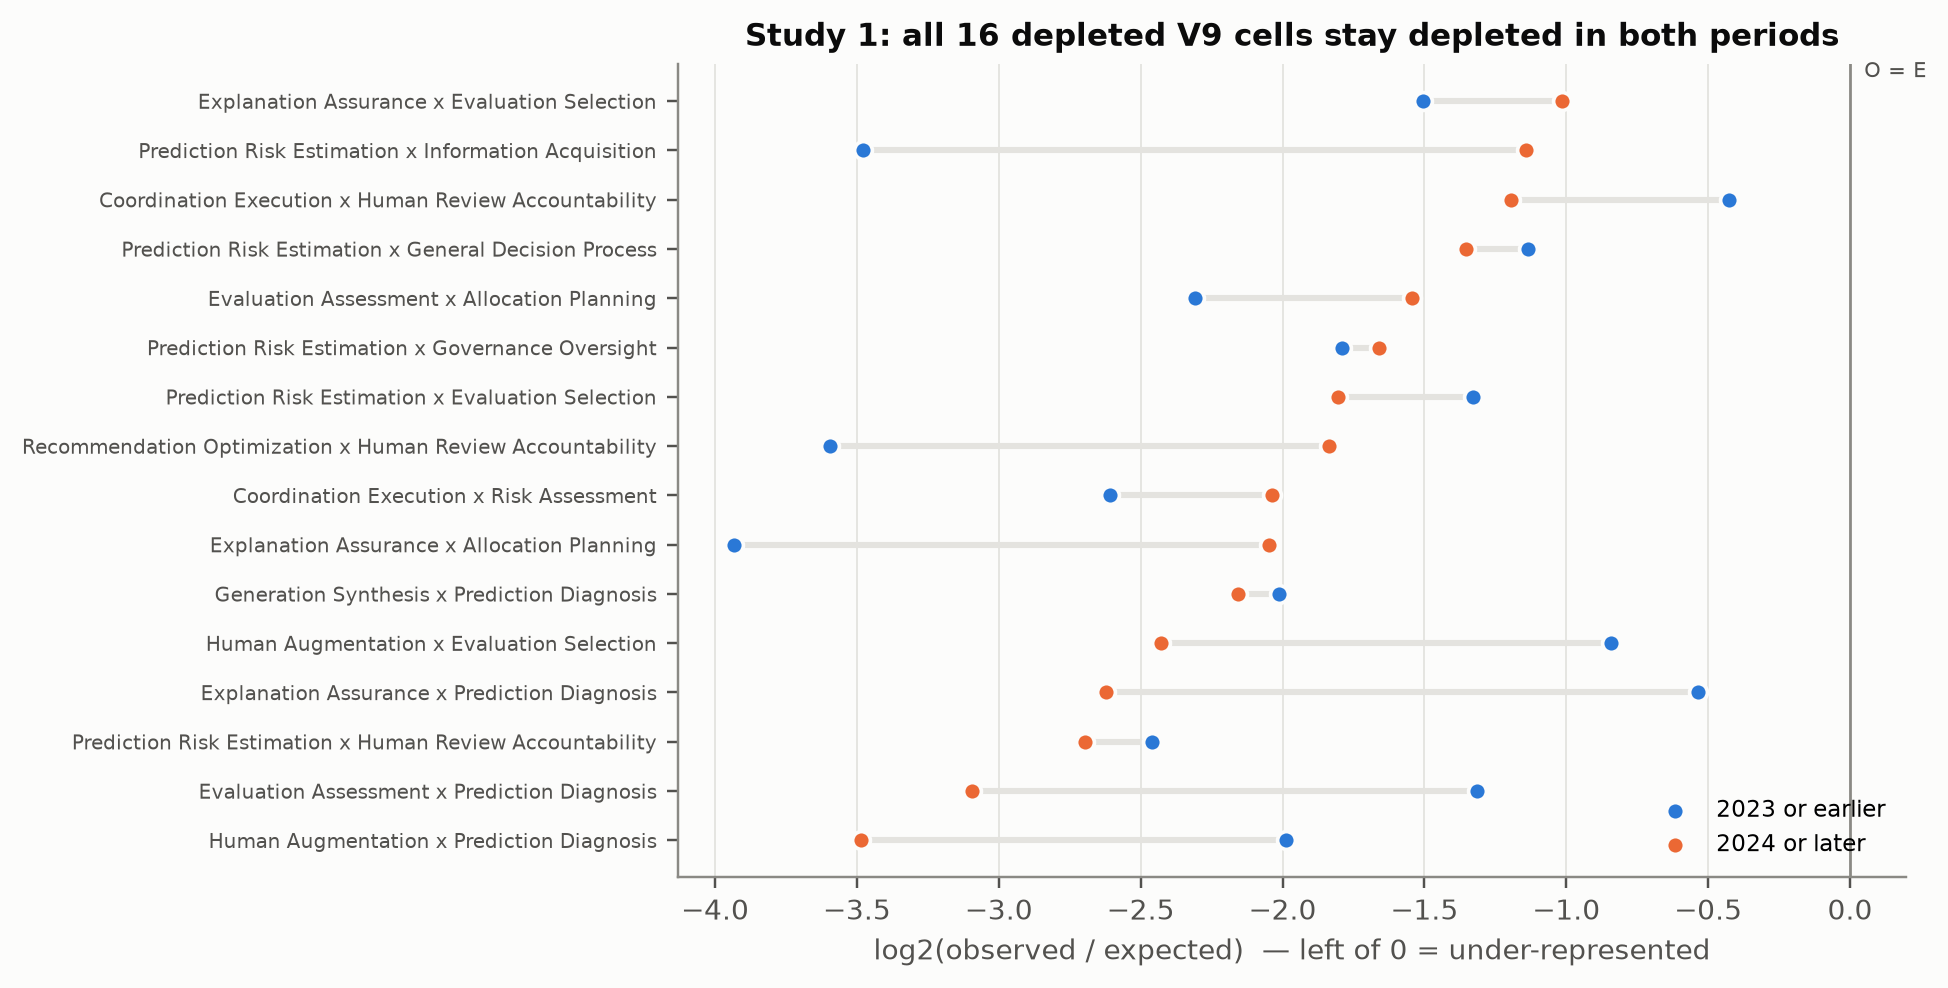
\includegraphics[width=\linewidth]{fig_study1_direction.png}
  \caption{研究一：16 個 V9 偏低格各自的 $\log_2(O/E)$，分別以 2023 年（含）以前（藍色）與 2024 年（含）以後（橙色）的文件計算。垂直線標示 $O = E$。各期的期望次數係以該期自身的邊際重新計算，故各期數值無法直接與合併計算的 O/E 比較（最極端格的合併值為 $O = 6$，$E = 44.9$）。此方向可能反映非隨機的編碼假象（第~\ref{zh:sec:study1_reliability}~節）。此為偏低格，而非缺口。DIRECT。}
  \label{zh:fig:study1_direction}
\end{figure}

\paragraph{三角檢證的限度。} 一旦編碼工具改變，方向的穩固程度便隨之降低：
\begin{itemize}
  \item 在關鍵詞（第一階段）編碼下，13/16 個偏低格維持相同方向。
  \item 同詞兩端共用（same-term self-pairing）膨脹了最強的偏高格（prediction $\times$ prediction）。該格中有 33\% 的紀錄在兩端配對同一詞彙（例如「forecasting」）。移除這些紀錄後，有 2 個與預測相關的偏低格退出核心格。
  \item 規則式關鍵詞矩陣移除 741 筆同詞紀錄，剩下 1,431 條文件邊。在此矩陣中，13/16 個偏低格維持相同方向，6 格顯著，0 格呈顯著反轉，但僅有 7 格進入四項檢定的核心格。
\end{itemize}
因此，偏低的方向對種子、來源軌與時期皆具穩健性，對關鍵詞編碼與移除同詞紀錄亦大致穩健。相對地，顯著核心格的組成則取決於句子的編碼方式。表~\ref{zh:tab:app_s1robust} 彙整所有穩健性檢查。

\subsection{測量信度與誤分類}
\label{zh:sec:study1_reliability}

表~\ref{zh:tab:reliability} 報告 AI 標籤與決策標籤經機遇校正的一致性（Cohen's $\kappa$；\citealp{cohen1960coefficient}）。

\begin{table}[tbp]
  \centering
  \small
  \caption{研究一標籤的編碼信度（Cohen's $\kappa$）。模型與模型之間的一致性僅顯示工具具可重現性，並非人工的評分者間信度（inter-rater reliability）。人工與人工之間的估計僅根據 $n = 20$ 筆紀錄，因此並不精確。DIRECT。}
  \label{zh:tab:reliability}
  \begin{tabular}{p{0.62\linewidth}rr}
    \toprule
    比較 & AI $\kappa$ & 決策 $\kappa$ \\
    \midrule
    人工 vs 人工（$n = 20$） & 0.05 & 0.14 \\
    處理流程 LLM（qwen）vs 第一位人工編碼者（$n = 50$） & 0.27 & 0.12 \\
    處理流程 LLM 再測（143 個標籤端） & 0.64 & 0.63 \\
    理論合併分類（7$\times$6），人工 vs 人工 & 0.08 & 0.16 \\
    兩個 Claude 模型，盲測，編碼手冊 v2（250 筆紀錄）：Sonnet vs Haiku$^{a}$ & 0.72 (0.87) & 0.56 (0.82) \\
    Claude（編碼手冊 v2）vs 協調後的人工答案（$n = 20$） & 0.45 & 0.70--0.76 \\
    處理流程 qwen vs 協調後的人工答案 & 0.11 & 0.29 \\
    \bottomrule
  \end{tabular}

  \smallskip
  \raggedright\footnotesize $^{a}$括號內為兩個模型皆有編碼之標籤端之間的一致性。
\end{table}

人工與人工之間的一致性極低，且僅基於 20 筆紀錄；改用較粗略的分類亦未見改善。處理流程在再測時穩定，但與人工編碼的一致性薄弱。兩個 Claude 模型之間的一致性較高，這顯示的是程序具可重現性，而非具可靠性。修訂後的編碼手冊也改變了被編碼的內容：在編碼手冊 v2 下，42--64\% 的證據句未陳述明確的決策功能，而處理流程的比例為 18\%；且僅約 9\% 的矩陣紀錄被兩位新編碼者重現於同一格中。

\paragraph{解析界限及其限度。} 令 $T$ 為一格在無誤編碼下的次數，$e_{\mathrm{AI}}$ 與 $e_{\mathrm{Dec}}$ 為兩個標籤的非差異性（隨機）誤差率。則
\begin{equation}
\frac{O^{\mathrm{obs}}}{E} - 1 = (1 - e_{\mathrm{AI}})(1 - e_{\mathrm{Dec}})\left(\frac{T}{E} - 1\right).
\label{zh:eq:attenuation}
\end{equation}
由於正確率乘積至多為 1，隨機誤差只會削弱偏低，而不會製造偏低。然而，此界限並不能保護方向，原因有二。

第一，此界限僅涵蓋非差異性誤分類（non-differential misclassification），而已記錄的兩項誤差來源並非隨機。同詞兩端共用膨脹了 prediction $\times$ prediction 格。在式~\eqref{zh:eq:s1_expected} 下，膨脹某一格會提高其所在列與欄的邊際，從而提高同列與同欄其他格的期望次數，使其 O/E 下降；因此，在固定邊際的矩陣中，編碼可能製造出偏低。本研究自身的移除證據限制了此一機制。在不含 741 筆同詞紀錄的情況下，13/16 個偏低格維持其方向，且無一呈顯著反轉；而自被膨脹的格中移除同詞配對紀錄，僅使 2 個偏低格退出核心格（第~\ref{zh:sec:study1_direction}~節）。因此，同詞兩端共用並非此型態的主要驅動因素。模型推論的標籤是第二個非隨機來源，且尚未經過檢驗：若模型將特定類型的句子導向特定家族，便會以有規律的方式在格與格之間移動紀錄。

第二，隨機誤差模型與資料並不相符。以最極端格而言，即使採用 95\% 上界，也需要正確率乘積至少為 0.71，而人工稽核所隱含的值約為 0.07。這指向非隨機誤差，或指向稽核規模過小而無法估計正確率；觀察到的幅度不應被解讀為人工編碼資料將會呈現的結果。

\paragraph{模擬。} 表~\ref{zh:tab:misclass} 在六種誤分類情境下重建矩陣，並重新執行 BH 精確檢定。當以任一人工編碼作為真值時，仍維持顯著之偏低格數的中位數為 0，儘管分別有 11 與 12 格維持其方向。僅最輕微的隨機誤差情境與 Claude 共識情境維持非零的中位數（7 與 4）。沒有任何情境產生虛假的偏低格，但模擬的誤差皆為隨機誤差，故此結果對非隨機誤差無法提供任何資訊。由於兩位人工編碼者在 20 筆紀錄上大多不一致，「作為真值」的情境屬於壓力測試，而非經校準的誤差模型。

\begin{table}[tbp]
  \centering
  \small
  \caption{16 個偏低格的誤分類模擬：每種情境執行 300 次。每次皆重建矩陣並重新執行 BH 精確檢定。表中數值為格數的中位數（第 5--95 百分位數）。所有模擬誤差皆為隨機誤差；「作為真值」的情境為壓力測試。沒有任何情境產生虛假的偏低格。DIRECT。}
  \label{zh:tab:misclass}
  \begin{tabular}{lll}
    \toprule
    情境 & 仍顯著 & 仍偏低 \\
    \midrule
    第一位人工編碼者作為真值 & 0 (0--1) & 11 (8--13) \\
    協調後的人工編碼作為真值 & 0 (0--1) & 12 (10--14) \\
    20\% 隨機誤差 + 20\% 刪除 & 7 (5--10) & 16 (15--16) \\
    40\% 隨機誤差 + 20\% 刪除 & 0 (0--1) & 14 (12--16) \\
    60\% 隨機誤差 + 20\% 刪除 & 0 (0--0) & 10 (7--13) \\
    Claude 共識（編碼手冊 v2）作為真值 & 4 (3--6) & 14 (12--15) \\
    \bottomrule
  \end{tabular}
\end{table}

2026 年 11 月 18 日的再分析記錄了四項判定：
\begin{itemize}
  \item 方向性的低整合（under-integration）：\texttt{DEFENSIBLE}；
  \item 「16 個統計上穩健的偏低配對」：依現行測量為 \texttt{NOT DEFENSIBLE}；
  \item Burt 結構洞：\texttt{STOP}，因此中介者（broker）搜尋予以終止；
  \item 研究缺口：\texttt{NOT SUPPORTED}。
\end{itemize}
本研究對第一項判定加以限定。此方向通過了本研究所能執行的每一項檢查，且同詞兩端共用無法解釋其大部分，但模型推論的標籤仍可能形塑了此方向。這是一個描述性、未經確認的型態，而「defensible」（可辯護）的意義僅止於此。

\subsection{網路分析脈絡 V6--V11.1 與 Gap Validity}
\label{zh:sec:study1_network}

研究一的歷次版本在引用網路、共同作者網路與高階網路中搜尋 Burt 式中介者（表~\ref{zh:tab:network_lines}）。根據這些 HISTORICAL／USER\_REPORTED 紀錄，沒有任何一條脈絡確認出中介者。V10.1 對 8 組候選配對的外部審查否證了其中 6 組，另有 2 組未能判定。V11.1 的身分與同儕驗證否決了 4 名候選者中的 3 名，並認定第 4 名的證據不足。

\begin{table}[tbp]
  \centering
  \small
  \caption{V6--V11.1 對 Burt 式中介者的網路搜尋。所有列皆為 HISTORICAL／USER\_REPORTED：取自先前的專案紀錄或由研究者報告，原始檔案未經重新驗證。}
  \label{zh:tab:network_lines}
  \setlength{\tabcolsep}{4pt}
  \begin{tabular}{l p{0.17\linewidth} p{0.33\linewidth} p{0.17\linewidth} l}
    \toprule
    版本 & 脈絡 & 規模 & 結果 & 等級 \\
    \midrule
    V6 & 引用 SNA & 458 條線索；13 名候選者 & 0 名確認 & HIST./USER \\
    V7 & 作者 SNA & 446 篇著作；8 名跨領域作者；2 名焦點候選者 & 0 名確認 & HIST./USER \\
    V8 & 引用擴充 & 1,111 篇施引著作；5,592 筆參考文獻 & 未確認 & HIST./USER \\
    V9 & 引用脈絡 & 3,983 篇探索著作 + 3,897 篇確認著作（共 7,880 篇） & 無確認的 Burt 結果 & HIST./USER \\
    V10 & 高階網路 & 14 名探索性候選者 $\rightarrow$ 8 組配對／7 名中介者 & 僅屬探索性 & HIST./USER \\
    V10.1 & 外部審查 & 8 組候選配對 & 6 組否證、2 組未定、0 組確認 & HIST./USER \\
    V11 & 共同作者 SNA & 26,443 名 V9 作者；30,140 名合併後作者 & 0 名確認 & HIST./USER \\
    V11.1 & 外部身分／同儕驗證 & 95 次 OpenAlex 查詢；檢視 7,880 篇著作；4 名候選者 & 3 名否決、1 名證據不足、0 名確認 & HIST./USER \\
    \bottomrule
  \end{tabular}

  \smallskip
  \raggedright\footnotesize SNA = 社會網路分析（social network analysis）。HIST./USER = HISTORICAL／USER\_REPORTED。
\end{table}

各脈絡所用的關係能承載的內容並不相同。共同作者脈絡（V7、V11）與高階脈絡（V10）建立在投影之上。共同作者網路是作者--著作隸屬資料的單模投影（one-mode projection）\citep{newman2001scientific}，因此共同發表一篇論文並非有方向的流動（flow）；即使資料完美無誤，這些脈絡也無法承載 Burt 的構念（第~\ref{zh:sec:theory_cooccurrence}~節）。引用脈絡（V6、V8、V9）則不同：引用原則上能承載有方向的流動，這也是研究二採用引用的原因。這些脈絡之所以失敗，是基於資料與設計上的理由：它們在文獻樣本中篩選候選中介者，而非針對經校準的虛無模型檢定群體層級的流動。以中心性為基礎的篩選，例如通過某一節點之最短路徑的比例 \citep{freeman1977set}，並不能確立中介（brokerage）；中介需要在具有群體成員身分的行動者之間存在有方向的開放二步路徑 \citep{gould1989structures}，而 Burt 所述的效益則建立在非冗餘的真實聯繫之上 \citep{burt1992structural}。

補充診斷 Gap Validity（DIRECT）記錄：全部 16 個偏低格在二分家族網路中皆有替代路徑（16/16），且網路限制度（Burt constraint）的間接項為零。兩者皆非實證證據：間接項為零對任何嚴格二分圖而言皆為恆等式（第~\ref{zh:sec:theory_cooccurrence}~節），而在 120 格中有 104 格有觀察值的情況下，替代路徑幾乎必然存在。此診斷僅明確指出：偏低格並不代表斷裂。

因此，研究一支持一項描述性主張：在此文獻中，依現行編碼，16 個偏低配對的共現（co-occurrence）頻率低於其邊際所隱含的水準，且在兩期中方向相同。此型態究竟屬於文獻本身或源自編碼，無法以這些資料判定。檢驗此前提需要有方向的流動，而這正是研究二所提供的。

% ======================================================================

\section{研究二：專利證據}
\label{zh:sec:study2}

研究二以有方向的知識流動（knowledge flow）檢驗此前提：即美國發明專利（utility patents）之間的申請人引用（applicant citation），並以審查員指派的 CPC 分類作為群體標籤。本研究是在六個公開的關係型資料來源未能通過流動效度關卡之後，才選定專利資料（第~\ref{zh:sec:design_sources}~節；表~\ref{zh:tab:app_sources}）。各項分析遵循第~\ref{zh:sec:design_prereg}~節所述的四份預先登錄計畫（表~\ref{zh:tab:app_prereg}）：這些計畫為自行加上時間戳記的提交（commit），其中僅計畫 1 早於所有專利結果，因此對於計畫 2--4，本研究主張的是其規則係事先固定，而非其研究問題係事先固定。各項偏離均以註明日期的修訂（amendment）記錄（表~\ref{zh:tab:app_amend}）。本節所有結果皆為 DIRECT。

\subsection{資料與整體檢定}
\label{zh:sec:study2_aggregate}

\paragraph{資料。} 本研究使用 USPTO PatentsView 的 \texttt{pvgpatdis} 資料表，下載日期為 2026 年 11 月 18 日 \citep{uspto2026patentsview}：包括 1976--2025 年核准的 8,512,829 件發明專利，以及 152,631,929 列引用資料；其中 87,414,291 列屬於分析範圍（施引年份 2010--2025），而這些引用中又有 63,083,371 列為申請人引用。引用被用作知識流動的代理指標 \citep{jaffe1993geographic}。由審查員加入的引用（examiner citation）可能無法反映發明人所知，因此主要設定僅使用申請人引用 \citep{alcacer2006patent}。由於 PatentsView 在 2013 年以前將非審查員引用標示為「cited by other」，此設定實際上涵蓋施引年份 2013--2025。

各群體採用核准年份 2010--2025：
\begin{itemize}
  \item AI（CPC \texttt{G06N}）：94,929 件專利；
  \item DEC（\texttt{G06Q10/04}，預測與最佳化；加上 \texttt{G06Q10/06}，資源、工作流程、管理與決策分析）：37,501 件；
  \item BRIDGE（兩者皆屬）：5,316 件；
  \item 其他商業方法專利（BIZ-OTHER；\texttt{G06Q} 但不含 \texttt{G06Q10}）：150,170 件。
\end{itemize}
跨群體計數排除橋接（BRIDGE）專利。

\paragraph{DEC 的構念效度。} \texttt{G06Q10/04}（預測與最佳化）在方法上與機器學習重疊，因此 AI--DEC 過度連結（over-connection）的一部分可能近乎機械性：兩個分類部分描述的是相同的技術。因此，此檢定所測量的是專利分類之間的技術鄰近性，而非 AI 融入管理決策的程度。構念效度（construct validity）仍未經檢驗。敏感度檢查 s2 將 DEC 擴大至整個 \texttt{G06Q10}，使強度 OE（見下文式~\eqref{zh:eq:oe}）由 3.05 降至 2.59，但判定不變（表~\ref{zh:tab:aggregate}）；然而 s2 仍包含 \texttt{/04}，因此只是稀釋而非隔離此一重疊。僅以 DEC = \texttt{G06Q10/06} 進行的分析，以及粒度相符的 H1a 參照集（見下文），本研究均未執行；兩者是未來研究最優先的穩健性檢查。領域層級的判定適用於此處所定義的 \texttt{G06N} 對 \texttt{G06Q10/04} + \texttt{/06}。

\paragraph{統計量。} 引用依 $s = $（施引專利核准年份，被引專利核准年份）分層。在每一層中，$\mathrm{out}_A(s)$ 為群體 $A$ 專利所做出的引用數，$\mathrm{in}_B(s)$ 為群體 $B$ 專利所獲得的引用數，$M(s)$ 為總數。時間分層的組態期望值（configuration expectation）為
\begin{equation}
E(A\!\rightarrow\!B) = \sum_{s} \frac{\mathrm{out}_A(s)\,\mathrm{in}_B(s)}{M(s)} ,
\label{zh:eq:patent_expected}
\end{equation}
而對稱的觀察對期望強度 OE 為
\begin{equation}
\mathrm{OE}(A,B) = \frac{O(A\!\rightarrow\!B) + O(B\!\rightarrow\!A)}{E(A\!\rightarrow\!B) + E(B\!\rightarrow\!A)} .
\label{zh:eq:oe}
\end{equation}

\paragraph{為何採用相對檢定。} 由於引用行為具有領域在地性，若採用絕對判準「$\mathrm{OE} < 1$」，幾乎任何一對領域都會被標記（第~\ref{zh:sec:theory_domains}~節）。在使用真實資料之前執行的合成校準顯示了這一點：在未植入結構洞時，$\mathrm{OE} = 0.388$，但檢定正確地回傳 \texttt{HOLE\_\allowbreak NOT\_\allowbreak SUPPORTED}；而在跨群體引用受到 30\% 或 50\% 抑制時，檢定能偵測出結構洞（表~\ref{zh:tab:app_oeyear}）。此生成器相當簡單（領域在地的引用加上植入的抑制），其無結構洞的基準線接近參照最低四分位數，而真實 OE 則遠高於此；此校準顯示的是從低基準線出發的偵測能力，而非在真實基準線下的檢定力。預先登錄的假說皆為相對假說：
\begin{itemize}
  \item \textbf{H1a：}$\mathrm{OE}(\mathrm{AI},\mathrm{DEC})$ 同時落在 $\{\mathrm{OE}(\mathrm{AI},X)\}$ 與 $\{\mathrm{OE}(\mathrm{DEC},X)\}$ 的最低四分位數 $Q_1$ 之內。參照集為 \texttt{G06}、\texttt{G16} 與 \texttt{H04} 中至少有 2,000 件專利的 179 個 CPC 大組（main group）。
  \item \textbf{H1b：}比值 $\mathrm{OE}(\mathrm{AI},\mathrm{DEC}) / \mathrm{OE}(\mathrm{AI},\mathrm{BIZ\text{-}OTHER})$ 小於 1，且其 95\% 信賴上界小於 1。
\end{itemize}
H1a 並未匹配粒度：DEC 由兩個 CPC 小組（subgroup）構成，而參照對象則為大組。範圍窄且同質的群體可能比範圍廣的群體呈現較高的 OE，因此 H1a 的百分位數可能偏向過度連結。本研究未計算小組層級的參照集。

\paragraph{結果。} 在主要設定下，$O = 30{,}843$，$E = 10{,}112$，得 $\mathrm{OE}(\mathrm{AI},\mathrm{DEC}) = 3.05$（95\% CI 2.94--3.17；以施引專利為群集的 Poisson 群集拔靴法，2,000 次重複）。兩個方向皆呈過度代表：AI$\rightarrow$DEC 為 $O = 21{,}820$、$E = 6{,}686$（O/E 3.26），DEC$\rightarrow$AI 為 $O = 9{,}023$、$E = 3{,}426$（O/E 2.63）。H1a 不成立：OE(AI,DEC) 高於 97.8\% 的 OE(AI,$X$) 值與 92.2\% 的 OE(DEC,$X$) 值，而最低四分位數門檻分別為 0.787（AI 側）與 0.502（DEC 側），中位數分別為 1.240 與 1.095。H1b 不成立：比值為 1.69（95\% CI 1.60--1.77），儘管比較配對本身亦呈過度連結（$\mathrm{OE}(\mathrm{AI},\mathrm{BIZ\text{-}OTHER}) = 1.809$）。預先登錄的判定為 \texttt{HOLE\_\allowbreak NOT\_\allowbreak SUPPORTED}。

全部六項預先登錄的敏感度分析（sensitivity analysis）設定皆與此判定一致（0/6 不一致；表~\ref{zh:tab:aggregate}、圖~\ref{zh:fig:patent_sensitivity}），因此依預先登錄的規則，此判定並不脆弱。OE 的範圍介於 2.59（s2，DEC 擴大至整個 \texttt{G06Q10}）至 4.25（s6，橋接專利於兩側皆計入）之間。

\begin{table}[tbp]
  \centering
  \caption{整體檢定：主要設定與六項預先登錄的敏感度設定。「相對 BIZ 比值」為 OE(AI,DEC)/OE(AI,BIZ-OTHER) 及其 95\% 拔靴法 CI。「百分位數」為 179 個參照值 OE(AI,$X$)／OE(DEC,$X$) 中被 OE(AI,DEC) 超過的比例。NOT\_SUPPORTED 為 HOLE\_NOT\_SUPPORTED 的縮寫。DIRECT。}
  \label{zh:tab:aggregate}
  \footnotesize
  \setlength{\tabcolsep}{4pt}
  \begin{tabular}{p{0.26\linewidth}rlll}
    \toprule
    設定 & OE(AI,DEC) & 相對 BIZ 比值（95\% CI） & 百分位數 AI／DEC & 判定 \\
    \midrule
    主要設定 & 3.05 & 1.69 (1.60--1.77) & 97.8\% / 92.2\% & \texttt{NOT\_\allowbreak SUPPORTED} \\
    s1 所有引用類別 & 3.00 & 1.65 (1.55--1.75) & 98.9\% / 92.7\% & \texttt{NOT\_\allowbreak SUPPORTED} \\
    s2 DEC = 整個 \texttt{G06Q10} & 2.59 & 1.43 (1.38--1.49) & 95.5\% / 89.9\% & \texttt{NOT\_\allowbreak SUPPORTED} \\
    s3 擴大 AI（+\texttt{G06F18}、\texttt{G06V10/70}） & 2.69 & 1.56 (1.50--1.63) & 94.4\% / 86.6\% & \texttt{NOT\_\allowbreak SUPPORTED} \\
    s4 僅限發明資訊（inventive）分類碼 & 3.00 & 1.62 (1.54--1.70) & 97.7\% / 94.5\% & \texttt{NOT\_\allowbreak SUPPORTED} \\
    s5 施引年份 2015+ & 3.04 & 1.69 (1.61--1.78) & 98.2\% / 92.9\% & \texttt{NOT\_\allowbreak SUPPORTED} \\
    s6 橋接專利計入兩側 & 4.25 & 2.35 (2.23--2.47) & 100\% / 99.4\% & \texttt{NOT\_\allowbreak SUPPORTED} \\
    \bottomrule
  \end{tabular}
\end{table}

\begin{figure}[tbp]
  \centering
  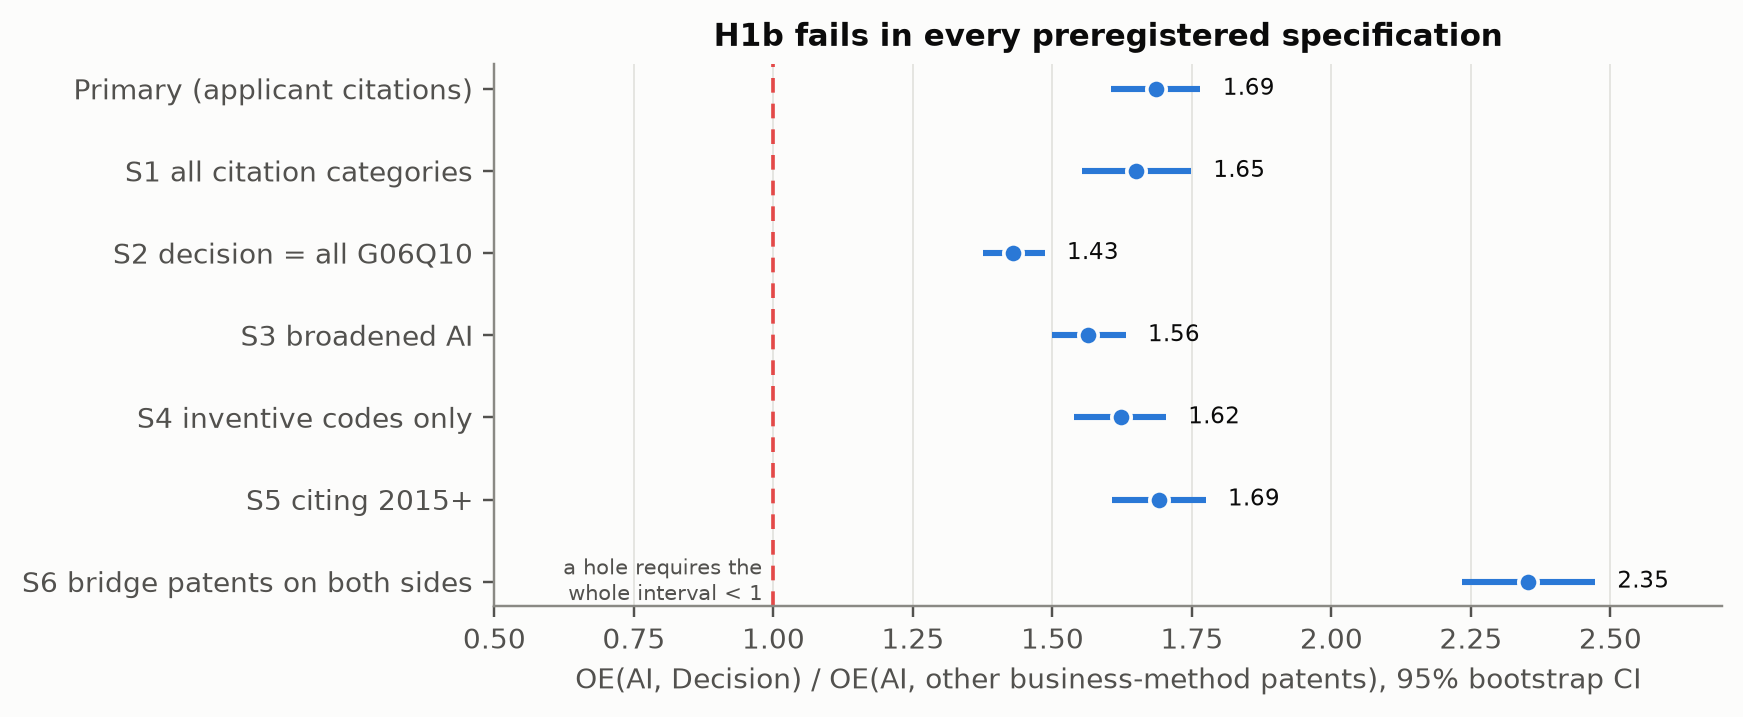
\includegraphics[width=\linewidth]{fig_patent_sensitivity.png}
  \caption{主要設定與六項敏感度設定下的 H1b 比值 OE(AI,DEC)/OE(AI,BIZ-OTHER) 及其 95\% CI。結構洞的成立要求整個區間皆落在 1 的虛線之下；每個區間皆位於其上。H1a 的百分位數見表~\ref{zh:tab:aggregate}。}
  \label{zh:fig:patent_sensitivity}
\end{figure}

\paragraph{趨勢（H2）。} 圖~\ref{zh:fig:patent_trend} 依施引年份繪出 OE(AI,DEC)。其值由 2013 年的 3.90 降至 2025 年的 2.34，加權最小平方斜率為每年 $-0.097$（95\% CI $-0.130$ 至 $-0.065$）。最近三年的 OE 為 2.69，而 DEC 側參照中位數為 1.095（AI 側為 1.240）。預先登錄的規則在斜率的 95\% CI 包含 0 或位於 0 以下時，將趨勢標記為 \texttt{PERSISTENT}，此處即屬後者。此規則原為結構洞情形而撰寫，在該情形中「收斂」意指 OE 朝參照值上升；套用於過度連結時，此標籤僅表示 OE 並未依該意義收斂，而非表示過度連結是穩定的。過度連結正在下降，但仍為 DEC 側參照中位數的兩倍以上。各年數值見表~\ref{zh:tab:app_oeyear}。

\begin{figure}[tbp]
  \centering
  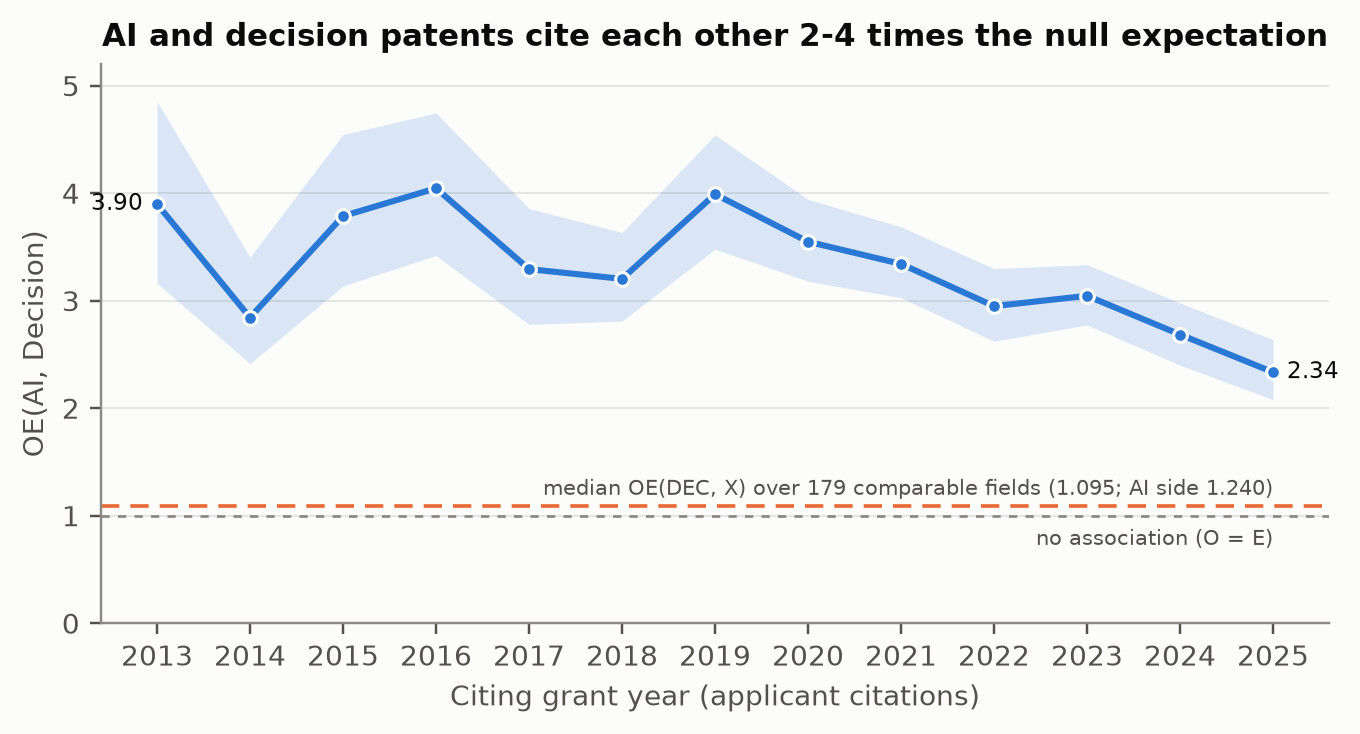
\includegraphics[width=\linewidth]{fig_patent_trend.png}
  \caption{2013--2025 年依施引專利核准年份計算的 OE(AI,DEC)，附 95\% CI 帶（僅申請人引用）。虛線為 DEC 側參照中位數，即 179 個可比較領域之 OE(DEC,$X$) 的中位數（1.095；AI 側中位數為 1.240），點線為 $O = E$。預先登錄標籤：\texttt{PERSISTENT}（斜率 CI 未高於 0；第~\ref{zh:sec:study2_aggregate}~節），儘管此序列呈下降趨勢。}
  \label{zh:fig:patent_trend}
\end{figure}

就 RQ1 而言，在此處的操作化定義下（\texttt{G06N} 對 \texttt{G06Q10/04} + \texttt{/06}），證據並不支持 AI 與決策技術之間的知識流動存在結構洞。這是在預先登錄規則下未能支持結構洞，而非證明不存在任何分隔；且過度連結的大小也不是組織整合程度的測量。

\subsection{CPC 矩陣上的 V9 檢定組與 M06-P 虛無模型}
\label{zh:sec:study2_cells}

預先登錄 2 將研究一的檢定組套用於功能矩陣的專利類比版本。此矩陣共有 42 格：
\begin{itemize}
  \item 6 個 AI 方法列：\texttt{G06N3}（神經網路）、\texttt{G06N5}（知識本位）、\texttt{G06N7}（機率／模糊）、\texttt{G06N10}（量子）、\texttt{G06N20}（機器學習）與 \texttt{G06N\_\allowbreak OTHER}；
  \item 7 個決策功能欄：FORECAST\_\allowbreak OPTIMISE（\texttt{G06Q10/04}）、RESOURCE\_\allowbreak SCHEDULING（\texttt{/0631}）、WORKFLOW（\texttt{/0633}）、RISK（\texttt{/0635}）、STRATEGY（\texttt{/0637}）、PERFORMANCE（\texttt{/0639}）與 MGMT\_\allowbreak GENERAL（其他 \texttt{/06}）。
\end{itemize}
所用引擎為 V9 引擎的位元組完全相同之複本（SHA-256 \texttt{09c3d60c\ldots bc33}）。此檢定組在三個部分上執行：
\begin{itemize}
  \item A 部分（Part A），共同分類：5,316 件專利與 14,573 條邊；
  \item B 部分（Part B），純 AI 專利與純 DEC 專利之間的申請人引用：30,843 筆引用與 66,056 條邊；
  \item 含所有引用類別的 B 部分：38,252 筆引用與 80,849 條邊。
\end{itemize}
由於 B 部分的 66,056 條邊來自 30,843 筆引用，第~\ref{zh:sec:study1_corpus}~節所述的群聚限制在此同樣適用。

\paragraph{退化的虛無模型及其替代。} 預先登錄的保留文件結構交換（M06）在 21,843,600 次提議的交換中接受了 0 次。原因是結構性的：每件專利貢獻其分類碼完整的列 $\times$ 欄乘積，因此每一個候選交換所指向的邊都已存在。預先登錄的核心格因而在建構上必然為空，對資料不提供任何資訊（修訂 B1，表~\ref{zh:tab:app_amend}）。其替代者為 M06-P（專利適用之保留文件結構虛無模型），它在（$|$列$|$, $|$欄$|$）分層內於文件之間置換欄集合，從而同時保留兩側邊際與每份文件的區塊結構（5,000 個樣本）。M06-P 是在 M06 失敗之後、且在三項檢定的格層級結果已知之後才設計的。它是對預先登錄 2 的有紀錄偏離，並在計算之前被凍結為預先登錄 3 的模組 P1；下文 M06-P 的結果即為 P1 的結果。M06-P 沒有獨立的型一誤差校準。

\paragraph{結果。} \emph{調整後完整核心}（adapted full core），即以 M06-P 取代 M06 的研究一核心規則，在 A 部分包含 8 個偏低格與 7 個偏高格，在 B 部分包含 9 個偏低格與 8 個偏高格，在含所有類別的 B 部分則為 8 與 8。各檢定（主要／精確／原始／M06-P）中 $q \le .05$ 的格數，在 A 部分為 20 / 20 / 29 / 22，在 B 部分為 22 / 22 / 27 / 25。表~\ref{zh:tab:cells_both} 列出在三項檢定一致（主要 + 精確 + 原始）下，於 A 與 B 皆偏低的五格，以及於兩者皆偏高的四格。依修訂 B1，三項檢定的結果屬探索性。圖~\ref{zh:fig:cpc_heatmap} 呈現完整矩陣。

\begin{table}[tbp]
  \centering
  \small
  \caption{在共同分類（A 部分）與引用流動（B 部分）中同方向偏離的 CPC 格。數值為 O/E，括號內為觀察／期望次數。偏低列：調整後完整核心（M06-P；預先登錄 3，模組 P1）與三項檢定一致給出相同的集合。偏高列依據三項檢定一致（主要 + 精確 + 原始），屬探索性（修訂 B1）。\texttt{G06N10}~$\times$~PERFORMANCE 屬小樣本（B 部分期望次數低於 10；A 部分整個量子列僅有 74 條邊）。此為偏低格，而非缺口。DIRECT。}
  \label{zh:tab:cells_both}
  \begin{tabular}{llll}
    \toprule
    AI 方法 & 決策功能 & A 部分 & B 部分 \\
    \midrule
    \multicolumn{4}{l}{\emph{A 與 B 皆偏低}} \\
    \texttt{G06N3} & RISK & 0.78 (171 / 219.5) & 0.70 (1,050 / 1,510.6) \\
    \texttt{G06N5} & RISK & 0.87 (255 / 291.9) & 0.85 (2,008 / 2,366.6) \\
    \texttt{G06N3} & MGMT\_\allowbreak GENERAL & 0.87 (497 / 572.7) & 0.95 (4,189 / 4,414.8) \\
    \texttt{G06N20} & FORECAST\_\allowbreak OPTIMISE & 0.89 (994 / 1,120.9) & 0.93 (2,255 / 2,425.9) \\
    \texttt{G06N10} & PERFORMANCE & 0.08 (1 / 12.0) & 0 (0 / 8.9) \\
    \midrule
    \multicolumn{4}{l}{\emph{A 與 B 皆偏高（主要 + 精確 + 原始；探索性）}} \\
    \texttt{G06N20} & RISK & 1.18 & 1.33 \\
    \texttt{G06N3} & FORECAST\_\allowbreak OPTIMISE & 1.09 & 1.17 \\
    \texttt{G06N5} & MGMT\_\allowbreak GENERAL & 1.16 & 1.06 \\
    \texttt{G06N7} & PERFORMANCE$^{a}$ & 1.15 & 1.16 \\
    \bottomrule
  \end{tabular}

  \smallskip
  \raggedright\footnotesize $^{a}$僅於 B 部分屬調整後完整核心（A 部分 M06-P $q = .93$）。
\end{table}

\begin{figure}[tbp]
  \centering
  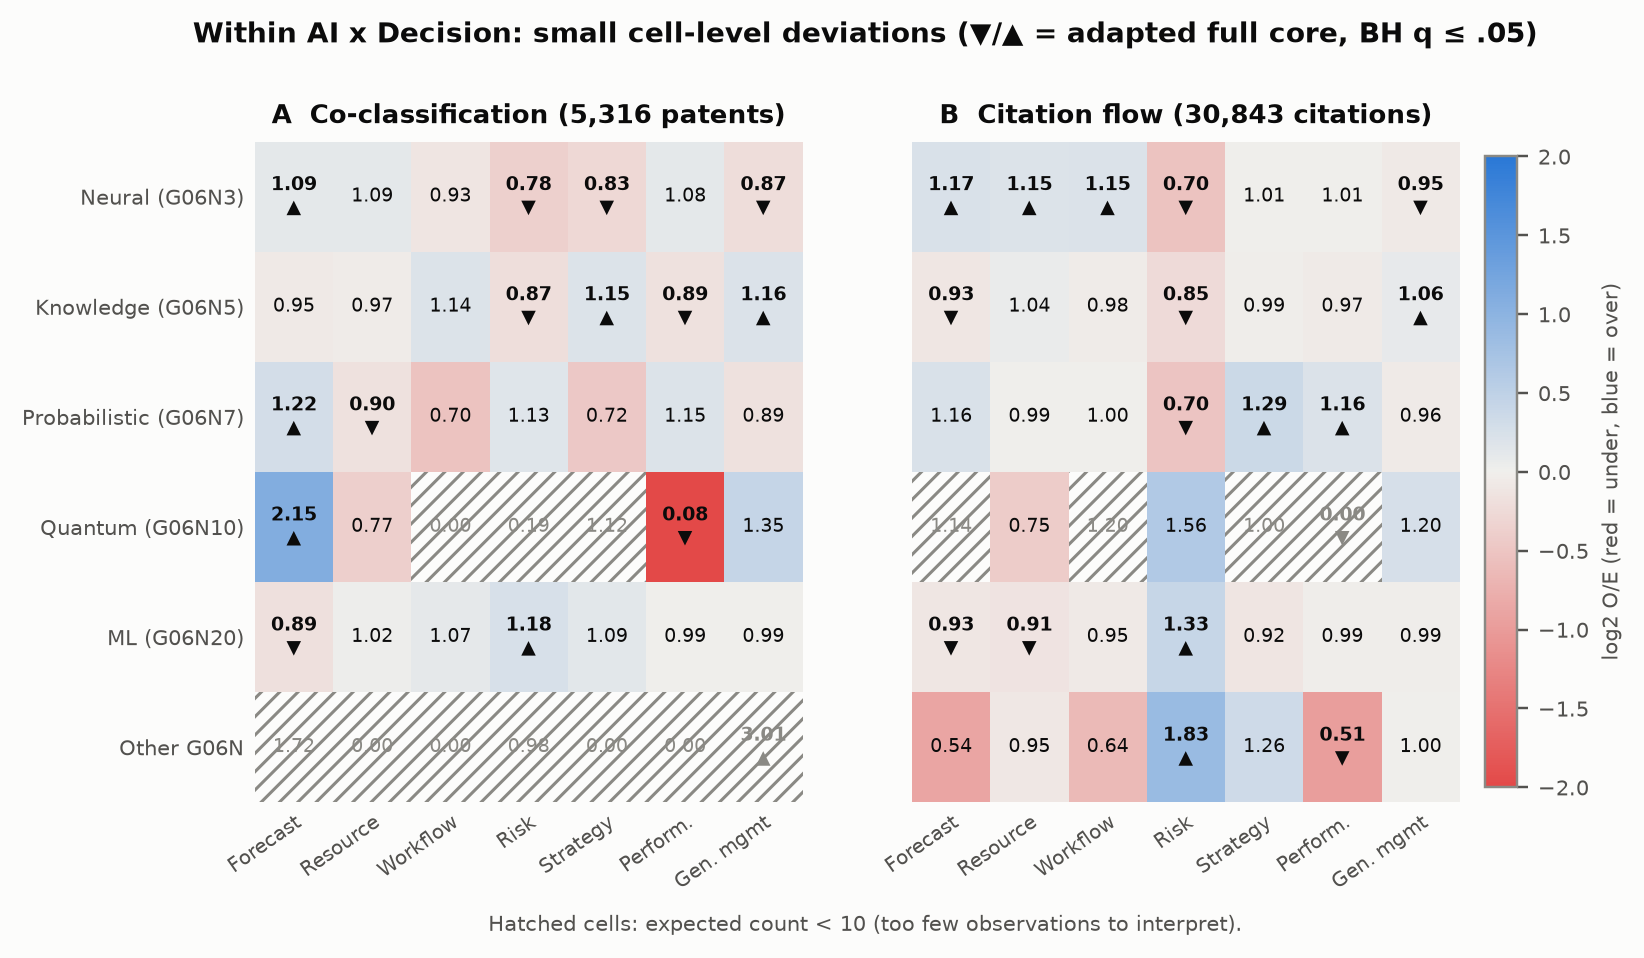
\includegraphics[width=\linewidth]{fig_cpc_heatmap.png}
  \caption{6$\times$7 CPC 矩陣中格層級的 $\log_2$ O/E：（A）共同分類，5,316 件專利；（B）申請人引用流動，30,843 筆引用。紅色表示代表不足，藍色表示過度代表。斜線格的期望次數低於 10，屬小樣本且不予詮釋，但仍予以呈現、在符合核心規則時加以標記，並納入下文的計數與表~\ref{zh:tab:cells_both}。三角形標示 M06-P 下的調整後完整核心（BH $q \le .05$；預先登錄 3，模組 P1）：A 部分為 8 個偏低／7 個偏高，B 部分為 9／8。\texttt{G06N7}~$\times$~PERFORMANCE 在 A 中沒有標記，因其僅於 B 部分屬調整後完整核心（A 部分 M06-P $q = .93$）。沒有任何偏低格在兩個時間半段中皆獲重現（第~\ref{zh:sec:study2_suite}~節）。}
  \label{zh:fig:cpc_heatmap}
\end{figure}

幅度比計數更為重要。除小樣本的量子格外，於兩部分皆偏低之五格的 O/E 介於 0.70 至 0.95 之間：這是在整體強度約為期望值三倍的領域配對內部的輕微不足。此範圍並未涵蓋 B 部分整個調整後核心：除量子格外，另有一個 B 部分核心格低於此範圍（圖~\ref{zh:fig:cpc_heatmap}）。這些格皆非分隔，本研究亦不將其稱為缺口。

\subsection{完整重現套組}
\label{zh:sec:study2_suite}

預先登錄 3 由十個模組 P1--P10 組成，每個模組為研究一的一條原始研究脈絡，在具流動效度的資料上提供一個專利類比。P1 即第~\ref{zh:sec:study2_cells}~節的檢定組。表~\ref{zh:tab:suite} 將 P2--P10 對應至其原始脈絡，表~\ref{zh:tab:app_suite} 則提供 P2、P3 與 P9 的細節。

\begin{table}[tbp]
  \centering
  \small
  \caption{完整重現套組：研究一原始脈絡的專利類比 P2--P10。DIRECT。}
  \label{zh:tab:suite}
  \setlength{\tabcolsep}{4pt}
  \begin{tabular}{l p{0.19\linewidth} p{0.24\linewidth} p{0.40\linewidth}}
    \toprule
    模組 & 原始脈絡 & 專利類比 & 結果 \\
    \midrule
    P2 & V9.1 校準 & 種子、虛無模型偽陽性率、檢定力、分段 & A：20 格恆為 $q \le .05$，4 格為邊界格；B：22 格恆為顯著，0 格為邊界格。每個虛無矩陣的平均虛假格數為 0.045（A）／0.049（B）。檢定力 67\%（A）／79\%（B） \\
    P3 & V6/V8/V9 引用脈絡 & 依時間半段進行探索／確認 & A：0 $\rightarrow$ 8 個偏低格（前半段僅 543 份文件）；B：3 $\rightarrow$ 11 個偏低格；0 個偏低格在兩個半段中皆獲重現 \\
    P4 & 研究一人工編碼稽核 & 標題關鍵詞標籤的表面效度（lift $\ge$ 1.5 即通過） & 全部 11 個標籤皆通過 \\
    P5 & V7/V11 作者 SNA & 含 Burt 限制度的公司引用網路 & AI\_FIRM$\sim$DEC\_FIRM O/E 0.24；符合預先登錄的公司層級判準（其後在專利組合虛無模型下為 \texttt{PARTIAL}）；MIXED 限制度中位數 0.36，度數匹配虛無模型為 0.444（$p = .001$） \\
    P6 & V10.1 外部審查 & 移除否證 & 10/10 名候選者被否證為不可或缺；最大聯合連通元件由 5,954 $\rightarrow$ 5,563 家公司 \\
    P7 & V10 高階網路 & 共同受讓超邊 & 2,546 條超邊；32\% 將一家 AI\_FIRM 與一家 DEC\_FIRM 或 MIXED 公司連結 \\
    P8 & V11.1 身分驗證 & 別名檢查 & 檢查 54 家公司；0 個可能的別名衝突 \\
    P9 & Gap Validity & 間接限制項；替代路徑 & 間接項為 0（對二分圖為恆等式）；每個偏低格有 20--30 條長度為 3 的替代路徑（在稠密矩陣中幾乎必然） \\
    P10 & Limitation Scout & --- & \texttt{NOT\_\allowbreak APPLICABLE}（專利沒有研究限制章節） \\
    \bottomrule
  \end{tabular}
\end{table}

\paragraph{P2：校準。} 在 20 個種子（$\times$ 10,000 次抽樣）下，B 部分的顯著集合完全相同（22 格恆為 $q \le .05$，0 個邊界格）；A 部分則有 20 格恆為顯著、4 格為邊界格。在 1,000 個端點置換虛無矩陣上（以 BH 校正的精確檢定），出現任何虛假格之矩陣的比例為 3.6\%（A）與 4.4\%（B）。這些虛無矩陣與精確檢定共享邊獨立的假設，因此無法揭露由文件內群聚所造成的反保守性。對於 $E \ge 100$ 的格，偵測 20\% 偏低的檢定力在 A 部分為 18/27 = 67\%，在 B 部分為 23/29 = 79\%，因此較弱或較小的偏低可能被遺漏。分段檢查見表~\ref{zh:tab:app_suite}。

\paragraph{P3：跨時間重現。} 偏低格數在 A 部分由 0（2010--2017）增至 8（2018--2025），在 B 部分由 3（2013--2018）增至 11（2019--2025）。無論在哪一部分，皆沒有任何偏低格在兩個半段中都獲重現。此處有兩點須注意。第一，A 部分的前半段僅有 543 份文件，檢定力不足。第二，P3 要求兩個半段皆出現顯著偏低，而研究一的時期檢查僅問方向是否維持。因此，P3 顯示的是格層級的顯著性無法跨時間重現；它並未顯示文獻型態比專利型態更為穩定。

\paragraph{P4：標籤表面效度。} 相對於其他 AI$\cup$DEC 專利，全部 11 個標籤在標題關鍵詞命中率上皆通過 1.5 的 lift 門檻；最低 lift 為 2.18（\texttt{G06N20}；所有 lift 值見表~\ref{zh:tab:app_lift}）。此檢查替代了研究一的編碼稽核，但它是標題關鍵詞檢查，而非人工稽核。

\paragraph{P5：公司網路。} 預先登錄 1 包含一項以領域層級結構洞為條件、關於受讓人（assignee）中介者的探索性 H3；由於 H1 未獲支持，H3 並未執行（修訂 A2）。P5 提出一個獨立的問題（RQ2）：無論領域層級的結果為何，公司（firm）層級是否存在結構洞；此模組在預先登錄 3 中被預先登錄為作者網路脈絡 V7 與 V11 的類比。經消歧的受讓人以申請人引用相連（排除自我引用），形成一個包含 6,201 個組織、20,681 條連結、總權重為 109,508 筆引用的網路。公司分為三組：2,926 家 AI\_FIRM（僅擁有純 AI 專利）、1,570 家 DEC\_FIRM 與 1,705 家 MIXED。群體 O/E 在 AI\_FIRM$\sim$DEC\_FIRM 為 0.24（$O = 886$，$E = 3{,}700$），在 AI\_FIRM$\sim$MIXED 為 0.81，在 DEC\_FIRM$\sim$MIXED 為 0.97。預先登錄的公司層級結構洞判準在此階段獲得滿足。Burt 限制度的中位數 \citep{burt1992structural} 在 AI\_FIRM 為 0.62，在 DEC\_FIRM 為 0.76，在 MIXED 為 0.36。相對於度數匹配的標籤置換虛無模型，MIXED 的中位數顯得偏低（虛無模型中位數 0.444；單尾 $p = .001$）。單獨來看，這正是此前提所預測的型態，但並非已確認的結構洞：標籤虛無模型固定了度數而未固定專利組合，此型態可能機械性地源自公司所擁有的專利。這一可能性促成了預先登錄 4。

\paragraph{P6：移除否證。} 度數至少為 5 且限制度最低的十家 MIXED 公司為 International Business Machines、General Electric、Tesla、ioCurrents、Google、Accenture、Amazon Technologies、T-Mobile USA、Optum Services 與 Strong Force VCN Portfolio 2019。移除全部 10 家之後，AI\_FIRM 與 DEC\_FIRM 公司仍然相連，且同時包含兩群的最大連通元件僅由 5,954 家縮減至 5,563 家：10/10 名候選者皆被否證為不可或缺的中介者。套組中的「跨群權重保留」指標在建構上恆等於 1，故本研究不據此做任何推論。

\paragraph{P7--P10。} P7（超邊）與 P8（別名）的結果見表~\ref{zh:tab:suite}。Gap Validity（P9）重複研究一的診斷：間接項為零是恆等式，而每個偏低格有 20--30 條長度為 3 的替代路徑，在稠密的 6$\times$7 矩陣中幾乎必然成立；兩者皆非證據。Limitation Scout（P10）是對論文所陳述之研究限制的檢查，不適用於專利。

\subsection{保留專利組合的公司虛無模型}
\label{zh:sec:study2_firm}

P5 的型態可能是機械性的。MIXED 公司同時擁有兩類專利，而專利主要引用其自身領域，因此即使沒有任何公司從事中介，位於不同領域的專門型公司（specialist firm）彼此之間的引用仍會很少。預先登錄 4 是在 P5 結果已知之後撰寫，並受其促成；其統計量、分層與決策規則則在計算任何一次重複之前即已凍結。其虛無模型，即保留專利組合的虛無模型（portfolio-preserving null），在分層內置換專利的擁有者集合，固定每家公司的專利組合與群體，以及整個專利層級的引用網路。主要分層為專利類型 $\times$ 核准年份（48 層）；技術組合分層（S-tech）為類型 $\times$ 年份 $\times$ AI 列 $\times$ DEC 欄（1,795 層）。每個虛無模型有 1,000 次重複，方案 $s$ 的第 $r$ 次重複使用種子序列 [20261119, $s$, $r$]。

\paragraph{範圍。} 此虛無模型以全部 127,114 件範圍內專利、擁有其中任一件的 14,600 家公司，以及其間的 162,339 筆申請人引用為起點。P5 僅報告移除自我引用後至少有一條公司間連結的 6,201 家公司（20,681 條連結；總權重 109,508）。恆等置換（每個擁有者集合皆保持原位）可精確重現 P5 的數值，因此兩組數字描述的是同一網路在兩個篩選階段的狀態。

\paragraph{虛無模型未固定之處。} 此虛無模型保留每家公司依類型與年份計算的專利組合件數，但未保留其度數或連結強度。限制度高度依賴度數 \citep{everett2020unpacking}，因此 T2 無法區分中介與度數。P5 的度數匹配標籤虛無模型（虛無模型中位數 0.444）與專利組合虛無模型（虛無模型中位數 0.104）回答的是不同的問題，且兩者皆未同時固定度數與專利組合。

\begin{table}[tbp]
  \centering
  \small
  \caption{保留專利組合的公司虛無模型：每種分層 1,000 次重複，附單尾（下尾）$p$ 值。T1 為專門型 AI 公司與決策公司之間連結的 O/E，T2 為 MIXED 公司的 Burt 限制度中位數。T1 符合其判準而 T2 不符合，因此兩種分層下的判定皆為 \texttt{PARTIAL}。此虛無模型並未保留公司度數。DIRECT。}
  \label{zh:tab:firm_null}
  \footnotesize
  \setlength{\tabcolsep}{4pt}
  \begin{tabular}{p{0.22\linewidth}rlrlr}
    \toprule
    & & \multicolumn{2}{c}{主要（類型 $\times$ 年份）} & \multicolumn{2}{c}{S-tech（+ 技術組合）} \\
    統計量 & 觀察值 & 虛無模型中位數 [95\%] & $p$ & 虛無模型中位數 [95\%] & $p$ \\
    \midrule
    T1 OE(AI\_FIRM$\sim$\allowbreak DEC\_FIRM) & 0.240 & 0.356 [0.317--0.398] & .001 & 0.307 [0.277--0.345] & .001 \\
    T2 MIXED 限制度中位數 & 0.358 & 0.104 [0.098--0.111] & 1.000 & 0.116 [0.110--0.122] & 1.000 \\
    OE AI\_FIRM$\sim$\allowbreak MIXED & 0.809 & 1.000 & .001 & 0.985 & .001 \\
    OE DEC\_FIRM$\sim$\allowbreak MIXED & 0.970 & 1.009 & .001 & 1.025 & .001 \\
    \bottomrule
  \end{tabular}
\end{table}

\paragraph{結果。} 結果見表~\ref{zh:tab:firm_null} 與圖~\ref{zh:fig:firm_null}。在兩種分層下，觀察到的專門型 O/E（T1 = 0.240）皆低於每一次虛無重複（$p = .001$，即 1,000 次重複所能達到的最小值）。然而，虛無模型中位數（0.356 與 0.307）本身即遠低於 1，且殘差的大小取決於所採用的尺度。在「與 1 之差距」的尺度上，固定專利組合的虛無模型重現了 T1 低於 $O = E$ 之觀察不足的 85\%（主要）與 91\%（S-tech），剩下 15\% 與 9\%。在比值尺度上，觀察到的專門型連結為虛無期望值的 0.240/0.356 = 0.67 與 0.240/0.307 = 0.78，即不足 33\% 與 22\%。兩種解讀皆屬有效，且回答的是不同的問題：專利組合能解釋與均等之間多少距離，以及真實連結比專利組合所隱含者低多少。專門型 AI 公司與決策公司之間的連結顯著少於其專利組合所隱含的水準；這並不表示有任何一方在兩者之間從事中介，本研究亦不將其稱為結構洞。

T2 未符合其判準。觀察到的 MIXED 限制度中位數（0.358）高於每一次虛無重複（虛無模型中位數 0.104 與 0.116；$p = 1.000$）：真實公司的群聚程度高於專利組合虛無模型所隱含者。由於此虛無模型未保留度數，此比較無法分離出中介。兩種分層下的判定皆為 \texttt{PARTIAL}，因此判定並不取決於技術組合。\texttt{PARTIAL} 表示「超越專利組合之組織結構洞」的雙判準規則並未滿足（表~\ref{zh:tab:app_prereg}）：公司層級的結構洞未獲確認。這並不表示結構洞已被排除，且 T1 已獲滿足。

\begin{figure}[tbp]
  \centering
  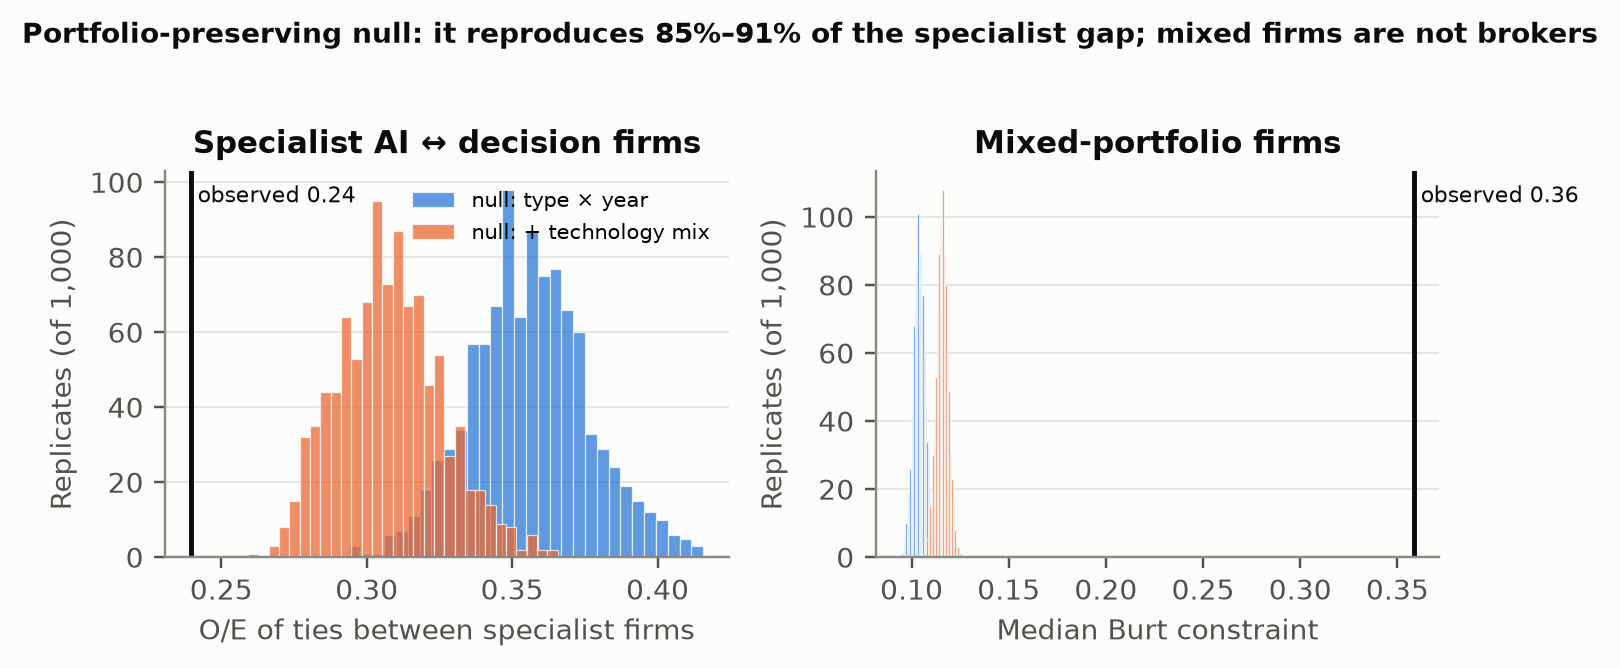
\includegraphics[width=\linewidth]{fig_firm_null.png}
  \caption{保留專利組合的公司虛無模型：在主要（類型 $\times$ 年份；藍色）與 S-tech（+ 技術組合；橙色）分層下各 1,000 次重複。專利組合、群體與專利層級的引用網路皆予固定；公司度數則未固定。左圖：T1，專門型 O/E（各 $p = .001$）；虛無模型重現了與 1 之差距的 85\% 與 91\%，而觀察到的連結為虛無模型中位數的 0.67 與 0.78（不足 33\% 與 22\%）。右圖：T2，MIXED 限制度中位數（各 $p = 1.000$）；此圖無法區分中介與度數，因此並未確立中介優勢。判定：兩種分層下皆為 \texttt{PARTIAL}；公司層級的中介仍未解決。}
  \label{zh:fig:firm_null}
\end{figure}

與 P5 的對比——相對於度數匹配的虛無模型，MIXED 的限制度偏低；相對於保留專利組合的虛無模型，則偏高——顯示虛無模型的選擇決定了對中介的解讀（第~\ref{zh:sec:discussion_measurement}~節）；由於專利組合虛無模型是受 P5 結果所促成，此一反轉屬於受資料啟發的後續分析。因此，RQ2 仍未解決。超越專利組合的專門型分隔是顯著的（兩種分層下皆為 $p = .001$），而 P5 的度數匹配虛無模型亦傾向 MIXED 公司具有較低的限制度（$p = .001$）；然而，沒有任何可用的虛無模型能同時固定度數與專利組合，因此混合型公司是否在此分隔中從事中介，無法在此判定。
